
\section{Discussion}
\subsection{Key Findings}
The most important takeaway regarding our main hypothesis is that the loss function that yields the best sound-matching outcomes varies depending on the synthesizer program. This is likely due to the interaction between how the parameters of the synthesizer influence the sound, and the core sonic features used by the loss function.

\textbf{Q1}: To what extent do automatic evaluation metrics agree with manual listening tests? 
\\We see somewhat consistent results between the rankings assigned by manual hearing tests (which we take as the ground truth), and automatic measures of P-Loss and MSS. With the exception of P-Loss in \BPNoise{} narrowly selecting a different spectrogram based loss, all measures of performance selected the same top performer. However, given the simplicity of our programs and the occasional deviations, we cannot conclude that these automatic measures are substitutes for human hearing tests. As many previous works have done (see Table~\ref{tab:summary}), the use of MSS and/or P-Loss as general loss functions does seem appropriate in general cases, however, the use of listening tests or custom made loss functions in specific contexts remains necessary. 

\textbf{Q2}: Are DTW and SIMSE effective measures of loss? If so, in what contexts?\\
\DTWEnv{} consistently outperformed other measures in amplitude-modulated synthesis, where envelope alignment is critical. \SIMSESpec{} performed best in subtractive synthesis, where scale-invariance captures noise-filtering effects more robustly than L1-based measures. These results suggest that the advantages of loss functions are context-dependent, underscoring the need for further exploration of creative differentiable similarity measures. 


\textbf{Q3}: Can iterative differentiable optimization be applied effectively with synthesizers using classical DSP functions? \\
The approach of designing DSP functions in Faust and transpiling to differentiable Faust code was convenient, yielded meaningful outputs, and enabled comparative evaluation of losses. We were able to run our 1200 experiments within 72 hours on a laptop without a GPU\footnote{Lenovo ThinkPad T480, i5-8350U CPU at 1.70GHz, 32 GB RAM.}.

\subsection{Practical Recommendations}
    Our findings not only provide answers to the research questions proposed in the introduction, but also serve as guidelines for practitioners in selecting appropriate similarity measures and synthesis methods for future experiments.
\begin{itemize}
    \item In lieu of listening tests, MSS or P-Loss are generally useful for large-scale benchmarking. However, we encourage confirmation of such results with manual listening, particularly if specificity is important. 
    \item For amplitude-modulated synthesis, DTW-based losses such as \DTWEnv{} are recommended over spectrogram differences and JTFS.
    \item  For subtractive/noise-filtered synthesis, spectrogram based losses are most effective. Based on our results, SIMSE appears to be the better method of spectrogram comparisons relative to L1, but the amplitude agnosticism of SIMSE likely plays a role in its poor performance in additive synthesis.  
    \item Iterative differentiable optimization via the Faust-to-JAX pipeline is a viable strategy for defining various differentiable DSP functions, requiring only modest hardware resources and providing a more natural approach to synthesizer definition.
    \item In our amplitude modulation experiments, \JTFS{} did not outperform other measures, contradicting prior claims of its superiority for mesostructures~\cite{vahidi2023mesostructures}. Thus, our results call into question its effectiveness as a general mesostructure measure, and highlight a need for further research into its utility.
\end{itemize}

\subsection{Illustrating Loss Landscapes}
\label{sec:loss_landscape_examples}
To complement our quantitative analysis, we provide examples of loss landscapes that illustrate why specific losses succeed or fail in certain synthesis contexts. These are illustrative aids rather than conclusive evidence, and highlight the importance of \PeriodicLoss{} discussed earlier in Section~\ref{sec:lacking}.

We show the landscapes of the loss functions with simplified versions of \BPNoise{} (HP-Noise) and \AmpMod{} (S-Noise-AM), each reduced to a single parameter for one-dimensional visualization. HP-Noise uses only a high-pass filter with cut-off between 100–20,000 Hz, while S-Noise-AM varies only the modulation rate between 0.1–20 Hz. Loss values are normalized to 0–1 to allow comparison across functions.

Figure~\ref{fig:loss_landscape_noisebp} shows the HP-Noise results. \LoneSpec{}, \SIMSESpec{}, and \JTFS{} exhibit clear minima at the correct parameter (red dashed line), whereas \DTWEnv{} remains relatively flat, making gradient-based optimization more difficult.

Figure~\ref{fig:loss_landscape_ampmod} shows the S-Noise-AM results. Here, \DTWEnv{} produces the smoothest and most informative landscape, while spectrogram losses are minimized near the target but lack consistent correlation with parameter distance. \JTFS{} remains largely flat. This aligns with \DTWEnv's superior performance in amplitude-modulated synthesis observed in our experiments.

\begin{figure*}[ht]
    \centering
    \begin{minipage}[t]{0.48\textwidth}
        \centering
        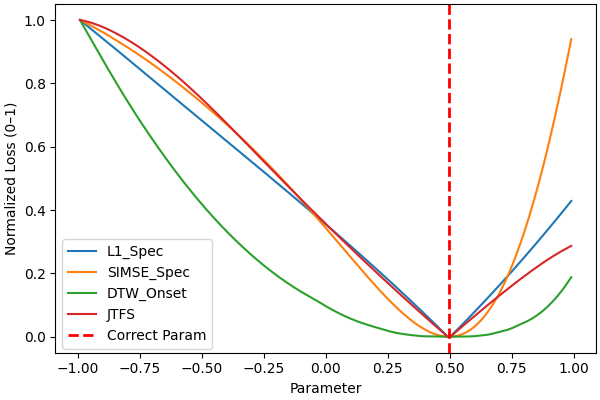
\includegraphics[width=\linewidth]{images/experiment_plots/comparing_loss_landscapes_normalized.png}
        \caption{Loss landscapes for \BPNoise{} with only a high-pass filter parameter. 
        \LoneSpec{}, \SIMSESpec{}, and \JTFS{} show clear global minima near the correct parameter, while \DTWEnv{} remains flat around the target.}
        \label{fig:loss_landscape_noisebp}
    \end{minipage}%
    \hfill
    \begin{minipage}[t]{0.48\textwidth}
        \centering
        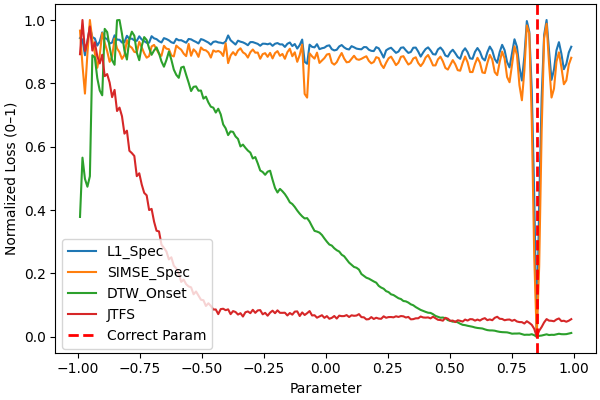
\includegraphics[width=\linewidth]{images/experiment_plots/comparing_lanscapes_1_1d_normalized.png}
        \caption{Loss landscapes for a simplified \AmpMod{} synthesizer with only amplitude modulation parameter. 
        \DTWEnv{} exhibits the smoothest and most informative landscape, explaining its superior performance in amplitude-modulated synthesis.}
        \label{fig:loss_landscape_ampmod}
    \end{minipage}
\end{figure*}


\subsection{Applicability to More Complex Synthesizers}
The experiments in this study were conducted with differentiable synthesizers chosen to isolate fundamental synthesis principles, each with two parameters. While this level of simplicity facilitates controlled comparisons, it does not fully capture the richness of real-world synthesizers, which can have hundreds of parameters with various routes. As a result, the extent of the generalizability of our findings does require further research. 

Nonetheless, we believe that the insights here can extend naturally to more complex domains. Depending on the feature of interest, the observed dependence of loss performance on synthesis method is likely to remain stable even with added complexities such as layers of modulation, filtering, or nonlinearity. 

\DTWEnv{} measures very specific features of audio, and its use in the recommended settings---where low frequency amplitude modulation matching is required---would likely yield the desired results regardless of synthesizer complexity. Likewise, the use of \SIMSESpec{} or \LoneSpec{} for matching filter cut-offs is likely to be successful regardless of the underlying sound. 

% Third, the iterative differentiable optimization framework proved viable even on limited hardware, which indicates that similar pipelines could be applied to larger differentiable synthesizers if computational resources allow.

% At the same time, real-world synthesizers present new challenges. 
% High-dimensional parameter spaces may exacerbate issues of local minima and make optimization less stable, particularly when loss functions are only partially informative. 


% Non-differentiable components (e.g., physical modeling, complex routing) also limit the direct applicability of gradient-based methods. 

\section{Summary, Weaknesses, and Conclusion}
\label{sec:summary_conclusion}
\textbf{Summary:} Sound-matching is an umbrella term for the algorithmic programming of audio synthesizers, often with the goal of assisting sound designers. Here we provided a history of sound-matching, major issues in the field, and discussed the importance of ``differentiable iterative sound-matching'' as a natural extension of current literature.

The main hypothesis tested here is whether the performance of differentiable loss functions is influenced by the synthesis techniques used for sound-matching. We conducted systematic iterative sound-matching experiments by combining four different loss functions with four different sound synthesis programs. We ranked the performance of the iterative sound-matching pipelines for every loss function and program, and observed that the success of the pipeline (that is, how closely the output sound matches the target sound) is program dependent. In other words, different synthesizer programs work best with different loss functions. Notably, we see that our novel use of DTW and SIMSE based differentiable loss functions (\DTWEnv{} and \SIMSESpec) can outperform what are regarded as the SOTA loss functions in 3 of 4 cases, although their success is highly synthesizer dependent. 

P-Loss and MSS have frequently been used as automatic performance measures, yet their ``preference'' has rarely been compared to human rankings. We observed that automatic performance measures and manual listening tests were generally in agreement, despite this, manual verification of sound-matching results remains a necessity in non-general experiments due to occasional divergences between automatic and manual tests.

\textbf{Weaknesses:} 
While we cannot prove that a universally best similarity measure does not exist, we can advocate for more creativity in the field. Compared to previous work, we presented a more cohesive approach to iterative sound-matching which utilizes a variety of loss functions and synthesis methods. However, there are many other methods of synthesis and sound-similarity that can be combined in practically infinite ways. Due to this large search space, we set arbitrary parameters for the various signal processing functions. We used bare-bones versions of STFT and JTFS with fixed parameters. We did not test complex synthesizers using parallel and sequential DSP functions. Arbitrary hyperparameters such as learning rate and max number of iterations were selected for the DL pipeline, and only the RMSProp optimizer was tested. 

 Like the majority of previous works, this work utilizes in-domain sounds; that is, the target sound is made by the synthesizer, and the parameters are already known. This simplifies the issues of measuring sound-similarity, but it is not a realistic scenario for practical sound-matching. This problem is left for future work, discussed in the next section.

\label{sec:future}
\textbf{Future Work: } The problem of periodic loss-landscapes, noted by many previous works, remains unaddressed~\cite{turian2020sorry,vahidi2023mesostructures,uzrad2024diffmoog,bruford2024synthesizer}. Perhaps this problem emerges due to the periodic nature of sound, which requires better loss landscape navigation methods. An optimizer that is more aware of fluctuations in the gradients would perhaps lead to better solutions than simple gradient descent. Viewing the sound-matching problem as ``the navigation of an agent from an arbitrary point in a gradient field to a target'' closely resembles many classical problems in the field of reinforcement learning (RL)~\cite{sutton2018reinforcement}. Naturally, the application of RL and other heuristic search techniques to the problem of iterative sound-matching would be an important contribution.

Contemporary works often involve the application of domain specific and computationally expensive loss functions~\cite{han2023perceptual,uzrad2024diffmoog}, use of large neural networks~\cite{hershey2017cnn,cramer2019look}, or complex ensemble methods~\cite{turian2022hear}. Such models are useful but intractable; furthermore, training them requires the definition of simpler loss functions, which emphasizes the need for further development of differentiable and expressive loss function implementations. 

Like nearly all previous work in sound-matching, the main measure of success here was the accurate \textit{replication} of sounds (or synthesizer parameters) rather than \textit{imitation} of sounds outside of the synthesizer's domain. Replication of arbitrary features of sounds is an important component of sound-design, though it is much harder to define or measure. Future works could explore loss functions which only measure certain characteristics of sound (such as \DTWEnv), and whether they can pave the way for better imitation in sound-matching.
